\documentclass[]{article}
\usepackage[margin = 1.5cm]{geometry}
\usepackage{url}

%smaller subtitle
\usepackage{relsize} 

%mutli line comments
\newcommand{\comment}[1]{}

%bibliography citations in order
\usepackage[numbers,sort&compress]{natbib}
\usepackage{graphicx}

%opening
\title{Fake News?
	\\ \vspace{2mm} \smaller[2]{}Fact-Checking Individual Statements With Web Scraping and Sentiment Analysis}
	%\\Fact-Checking Individual Statements With Web Scraping and Sentiment Analysis}
\author{Sofia Escoto}

\begin{document}
	\maketitle
	
	\section{Introduction}
		
		%week2 assignment
		%1.1. Introduction - state your goal and hypothesis, why it is original and why nobody solved it before (10p)
		
		The spread of misinformation is a large societal problem, exacerbated by the widespread use of social media. Today, anyone can log into their computer and say something that the entire world can see. While the malicious spread of misinformation is  often seen in regards to politics, it's not exclusive to it, and though anyone with a computer can also access a search engine and tell if a statement is false based on the results, it's rare that a person will take the time out of their day to do so. Because of this, many people spread false, and potentially harmful, statements online due to ignorance.
		
		With a machine learning algorithm that takes a statement (ex. a blue whale can weigh up to 200 tons) and classifies the statement as either true or false, a person doesn't have to take any time to Google it on their own. With this model used in conjunction with or integrated into websites like Twitter, Facebook, and Reddit, misinformation could be easily recognized as false and therefore would be unlikely to ``go viral" and spread to more users. 
		
		Though machine learning has been used before for fact-checking and determining the credibility of a claim, most of its application has been in analyzing either full-length articles using context clues and sources or on subjective statements that were trained to use `common sense'. Obtaining truth values of objective statements has not been previously attempted in the public sphere, (i.e. outside of scientific claims \cite{wadden20}) or without significant amounts of pre-validated data available (i.e. as a part of a broader algorithm with a question-and-answer input-output model that relies on fact databases \cite{lazarski21}).
		
		 With this proposed model, the truth values of objective statements will be available with a single click to ordinary Internet users, who may have otherwise just taken whatever they read online at face value.
		
		
	\section{Literature Review}
		
		%1.2. Literature review - describe similar work that has been done, with references, and where that work failed short of answering your question (10p)
		
		Most often when a person wants to know whether something online is true or not, they're concerned with political articles. Using machine learning to analyze fake news (which is defined as any article that is ``intentionally and verifiably false") has been studied widely in recent years, using context, word usage, and sources determine credibility \cite{shu19}. This is very useful when dealing with long-form journalism, but isn't applicable for finding truth values of individual statements. Because a large part of this method involves analyzing the source the article came from, any lone statement from social media sites like Twitter or Facebook would be at a disadvantage. Alternatively, if attempting to fact-check a single sentence in an article, the truth value of this statement may not match up with that of the article as a whole, and could lead to inaccurate results. 
		
		Other research being done in this sphere, especially considering individual sentences, are essentially trying to get machines to use `common sense.' Some of these models aim for the computer to `understand' a given sentence, taking meaning from it and allowing a user to get the gist of a claim without needing to know exactly what was said. This can include determining the emotional connotation of a sentence, classifying opinions and reviews as negative or positive, or categorizing sentences based on broad subject matter. These models can start without prior knowledge of words and their meanings, only given an alphabet and large training set \cite{zhang15}, or build off of individual words and their definitions in addition to grammatical rules \cite{wang05}, because they rely on previous experience. This means that simple, common-sense statements can be analyzed with relative ease, but statements that require more than just reasoning can not.
		%When using CNN's for these purposes, models can `perform remarkably well' with only one layer of convolution \cite{kim14}. 
		
		The most relevant research to the proposed model is about fact-checking and trying to determine the truth value of individual claims as described in \textit{Using NLP for fact checking: a survey}. In this procedure, though, the algorithm must first determine whether the statement given is a claim at all. Because this seemed outside the scope of 5-week course and, ``though research has gone into claim detection, there is no formal definition of what a claim is yet \cite{lazarski21}," this step will not be included in the proposed model. Once a statement is confirmed to be a claim and is therefore able to be fact-checked, the algorithm searches through a fact database that stores prior claims that have already been manually fact-checked by experts. If the database does not have the information needed, the Internet can be utilized, in some situations just returning a snippet of the first search result to the user, and in other cases using sentiment analysis on the results to determine the credibility of the claim. Search results that include unassertive words can suggest a false claim, as well as the use of first and second person pronouns as opposed to third person. When trying to fact-check a claim that is not included in a given fact database, ``methods that utilize powerful search engines on the Internet perform best \cite{lazarski21}."
			
	
	\section{Data}
	
		%1.3. Add a link to the dataset/s you plan to work with (must be open source); if the dataset is not very big, you are also welcome to submit it here on Blackboard or on your Github repository (5p).
		
		Since there isn't an open-source dataset of statements with truth values, I decided to create my own by scraping trivia websites and articles that tell the user whether a statement is true or not. When I have enough claims, ideally at least 500 instances, I would use an API to enter the statement in a Google search and scrape the results for `snippets' to input into the dataset as well \cite{k_api}. Once added to the dataset, cleaning will include removing markdown commands.
		
		%week3 assignment
		%2. Continue your technical report (you are welcome to submit the same as you did last week or a revised report if I asked you so, plus the following):
		
		%2.1. first exploration of the data (summary statistics, number of variables, which are the variables of interest, which you will discard, etc.) (10p)
			
		Using the bs4 package in python and multiple websites (\cite{tf1}, \cite{tf2}, \cite{tf3}, \cite{tf4}, \cite{tf5}, \cite{tf6}, \cite{tf7}), I gathered 573 statements and their truth values. My original goal was 500 statements, but because I did not manually check for similarities, 573 gives a good margin of error in case there are duplicate statements from two different websites. Then I used an API to scrape Google and collect the "featured snippet" that comes up when the claim is searched, the descriptions from the first 10 results, and the number of results that come up in the search \cite{a_api}
		% 
		\footnote{Note that I used a different API for this initial scrape than I planned to use when constructing a web app to deploy the model. This is because this API allows for 1,000 searches per month which is convenient for populating a large dataset all at once, and the other API allows for 100 searches per day which is convenient for an app, where fewer searches will be made more often.}. 
		%
		This gave me a total of five features, four of type string (`statement', `snippet', `description', `results') and one of type boolean (`truthValue').
		
	\section{Methods}
		
		%2.2. the methods you are using and why you are choosing these methods for the goal you stated in Week 2 (10p)
		
		%2.3. discuss the the pros and cons for the methodology (5p).
		
		%Research has shown that using CNNs in NLP is very beneficial \cite{kim14}. Human language is much more complex than classes like yes/no or numbers like integers/floats, and CNN's pooling ability allows for dimension reduction and the analysis of very complex data. With my research, this will be entirely necessary; the 'description' feature in this dataset, for example, has an average of over 1300 characters in each instance. Besides the technical benefits of CNNs, the implimentation in python with TensorFlow is widely documented online and will be easy to trouble-shoot if I run into problems. Though CNNs can be very computationally expensive, they usually return more accurate classifications than other less complex machine learning models, which is very important to me in this project.
		
		I hope to classify these statements using a K nearest-neighbors algorithm. K nearest-neighbors (KNN) compares an instance to k other instances that are closest to it, aka its `neighbors.' Because of KNN's simplicity and ease of use, this seems like a good option. Although KNNS can be slower than other algorithms and suffer from the curse of dimensionality (slowing down significantly as more features are considered), because I don't have a very large dataset or very many features to test, I think I will be fine.
		
		A KNN model that could use non-categorical and non-numerical features was not included in scikit-learn's base packages, so with the help of the Towards Data Science website \cite{tds} I created my own algorithm for the purposes of natural language processing. The simplicity of KNNs was very useful here, because I otherwise may not have understood how to implement the process in my own code. This method does have the drawback of being slower than other models, especially considering that I relied on a naive solution of nested for loops when building  many of the functions in the class.
		
		
		%feedback
		%CNNs and NLP are two very different things. Actually CNNs are better for image analysis and computer vision than for NLP. You don't have the time to use all of these methods.For classification purposes, you are better off in this case with a simple kmeans algorithm.
		
		%For EDA, include the summary of the data that you scrapped and a data dictionary (which are the variables you are ultimately working with and what they represent).
		
	\section{Results}
	
	
		%3.1. final results of your data analysis; these should be included in your GitHub repository as well, therefore submit the link to GitHub too (10p)
		%3.2. description of the methodology you used and why (rationale) (10p).
		%3.3. preliminary visualizations of your results (5p).
	
		
		Using seven public websites with true/false questions, I scraped both the questions and their truth values into a dataset, giving me 573 instances. Once the questions and truth values were set in the dataset, using an API I scraped Google to give a summary of what the search for each question would bring up, the number of results, and the descriptions of the first ten sites in the search. A data dictionary is as follows:
		
		\begin{itemize}
			\item question: (type: string) An objective true or false statement. Ex. \texttt{Most people have 12 toes}
				
			\item truthValue: (type: boolean) A boolean value that corresponds to the question in its instance. Ex. `most people have 12 toes' as a question would result in \texttt{FALSE} as a truthValue.
				
			\item snippet: (type: string) A one-sentence description that Google provides after searching the question in its instance. Ex. there will be no snippet that results from the question `most people have 12 toes,' meaning the value in this instance will be \texttt{None}
				
			\item description: (type: string) A collection of the first 10 descriptions that show up in a Google search of the question. Ex. the description in this variable for the question `most people have 12 toes,' begins with \texttt{Be it a baby born with 12 toes and 12 fingers or a girl with elf-like ears, some people are just so special, they stand out from the crowd without trying. Its almost as if Mother Nature was feeling too creative when she created them.} and carries on to have 9 other similar sentences
				
			\item results: (type: integer) The number of results that Google will come up with after searching the question. Ex. `most people have 12 toes' will return \texttt{1772}| results.
		\end{itemize}
		
		\begin{figure}
			\centering
			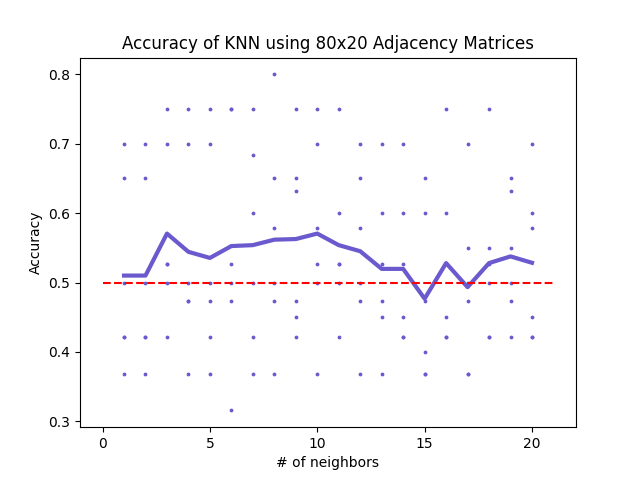
\includegraphics[width=0.8\linewidth]{accuracies-line.png}
			\caption{Scatter plot of the accuracy for models using k = 1-40 and plotting the mean of each k in purple. A red line at 50\% shows the cut-off for the model being less-accurate than guessing at random.}
			\label{fig:scatter}
		\end{figure}
		
		\begin{figure}
			\centering
			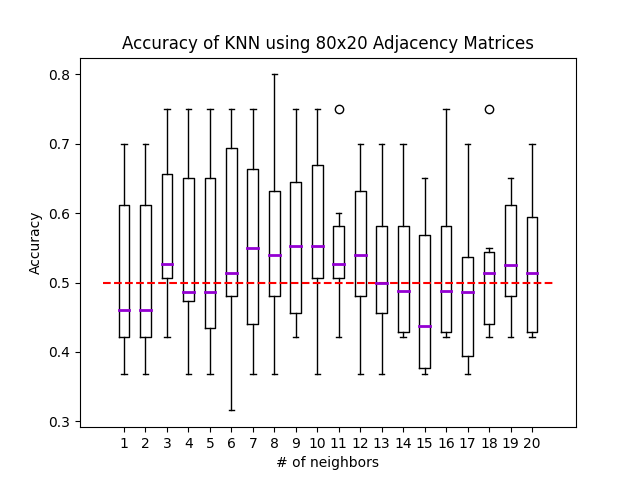
\includegraphics[width=0.8\linewidth]{accuracies-box.png}
			\caption{Box plot of the accuracy for models using k = 1-40 with the median shown as a purple line. A red line at 50\% shows the cut-off for the model being less-accurate than guessing at random.}
			\label{fig:box}
		\end{figure}
	
		I created my own user-friendly KNN algorithm (as seen in \texttt{model.py}) that used the nltk package to compare statements and store their similarities in an adjacency matrix. Using this matrix, I was able to predict truth values of the same statements using different values of k, allowing me to see the number of `neighbors' that gave me the best results without repeating any calculations.
		I was able to achieve a mean accuracy of 58\% at k = 20 that continued comparably all the way up to k = 40 (shown in figures \ref{fig:scatter} and \ref{fig:box}) which I believe is sufficient considering the scope of this class and my access to computational resources.
		
		
		With more computing power, I'm confident that I could increase the accuracy of this model by at least 15\%. One reason that the accuracy is so comparatively low is because, in order to get results in a reasonable amount of time, I had to partition the data into 6 segments so as to create six 80x20 adjacency matrices (requiring knn.process() to compare 9,600 text statements) as opposed to one 480x120 matrix that would require 57,600 comparisons. Comparing 9,600 segments and saving the results took over two hours on my PC, so although the accuracy would be improved with a broader training set, attempting this would not have been realistic.
		
		Once the adjacency matrix has been calculated, however, knn.predict() takes a very short time to output results since it uses the same matrix for all values of k, so long as the training and testing set stay constant. If I had access to a computer that could run for 12+ hours uninterrupted, I would be able to run knn.process() and then analyze my entire dataset at once, with the option of using even more data by scraping some additional websites.
		
		
		%feedback
		%What is the accuracy of KNN? It's not included here. Also, you need to populate the Readme page from GitHub with details of your project. Additionally you need to include visualizations of the results.
		
		
		
		
		%week5
		
		%4.1. Final techincal report that includes the goal of the project (2p), the literature review (2p), the description of the data (3p), the description of the methods (3p), the results (3p) and the visualization of the results (3p). (total 16p).
		%4.2. The GitHub repository link where you describe succintly your project on the first page (2p), you include the dataset and/or an open link to the dataset (2p), and your clean and commented code, that is running (5p). (total 9p).
		
	\bibliographystyle{unsrt}
	\bibliography{492}
	%if gets out of order - style = unsrtnat
\end{document}



%intro planning.... ignore!!!

\comment{
	What is the problem?
	Why is it interesting and important?
	Why is it hard? (E.g., why do naive approaches fail?)
	Why hasn't it been solved before? (Or, what's wrong with previous proposed solutions? How does mine differ?)
	What are the key components of my approach and results? Also include any specific limitations.
	\bibliography{technical paper}
	
	question: is it possible to determine whether an individual statement (given no other context) is true or false with 80\% accuracy?
	
	goal: determine whether a statement found online can be trusted without making the user go and look it up and determine for themselves
	
	h0: it is not possible to predict the accuracy of common statements with 80\% accuracy or above through simple web scraping and sentiment analysis
	
	h1: it is possible to predict the accuracy of common statements with 80\% accuracy or above using simple web scraping and sentiment analysis.
	
	original because most fake news models are focused solely on political content and scanning website credibility, not focusing on general facts and figures. hasn't been solved before bc it's easy to find these answers with a google search. it's still important, though, because most people DONT go find the answers, simply take them at face value
	
} 


%lit review summaries.... ignore!!!!

fake news - pdf on desktop - shu19
- fake news can be described as any "news article that is intentionally and verifiably false." (introduction pg 18 ?)
-use cnn's with the text and source to determine credibility and see if the article as a whole is 'fake news'. if there were one false statement, the entire article would be classified as false and while this is good for someone who wants to know whether or not to trust an article, it's not if someone wants to know if a specific statement is true or false. If the answer is false, the statement may be true and simply share a page with a false statement, entirely separate from itself.

experience based - wang05
- uses semantics and study of formal languages
- adaptive, must have memory and looks for answer  that is 'most consistent with its experience under the restriction of available resources'
-inheritance statements relates two concepts, for example bird and raven, and this model uses its experience to relate the terms. if the sentence said 'a raven is a bird' NARS, if given enough resources to connect the two terms, will set the truth value of this statement to true. this means that simple, common-sense statements can be found out with relative ease, but more complex statements that require specific knowledge and not just reasoning can not.

text understanding from scratch - zhang15
-understanding the general meaning behind a sentence given using matching words and classification
-cnns
-doesnt require knowledge of syntax or words, uses context and an input alphabet for the language and then prepared into vectors (words). a dictionary doesnt need to be inputted beforehand
-similar as others, sentiment analysis (good/bad), subject categorizing - only 'for its semantic or sentiment[al] meaning.'

cnns for sentence classification - kim14
-nlp used with statements that are not necessarily (though can be) claims, and instead of finding truth values will classify the statement according to its sentiment (whether a statement is good or bad, rating a review on a scale of positive to negative, or separating sentences by their subject matter)
-found that cnn's with just one layer of convolution 'perform remarkably well' for such purposes

fact checking with nlp - lazarski21
-n-grams to group n amount of words
-neural networks
-statements must be verified as being a claim and not an opinion, joke, etc. which means another step in the process of fact checking. 
-'Inconveniently, even though research has gone into claim detection, there is no formal definition of what a claim is yet.'
-claims can be compared using fact databases that have been pre-fact checked by professionals, the internet (if a fact database fails) using the first snippet result of a google search to show the user
-sources can be trusted also based on sentiment analysis. unassertive words might mean a false claim, as well as first and second person pronouns (I, me, you, yours) as opposed to third person pronouns (he, she, they), or exaggerated words in lieu of numerical data.
-'regarding generalized fact checking, methods that utilize powerful search enginges on the internet perform best.' the challenge is getting fact checks on things that humans have not previously looked at and things that aren't already in fact-databases
